% Tipo de documento
\documentclass[12pt, twoside, a4paper, openany, bibliography=totoc, numbers=noenddot]{scrbook}

% Añadir caracteres no anglosajones como tildes, ñ, ¿, ¡, etc.
\usepackage[utf8]{inputenc}
\usepackage[spanish]{babel}
 
% Añadir gráficos
\usepackage{graphicx}
% Carpeta donde se encuentran las imágenes
\graphicspath{ {figs/} }
\usepackage[labelfont=bf]{caption}
\usepackage{subcaption}
\DeclareGraphicsExtensions{.pdf,.png,.jpg}
\usepackage{chngcntr}
\counterwithout{figure}{chapter}

% Listas con corchetes tipo [1], [2]...
\usepackage{enumitem}

% Permite usar hipervínculos
\usepackage[hidelinks]{hyperref}

\usepackage{afterpage}

\newcommand\blankpage{
    \null
    \thispagestyle{empty}
    \newpage}

% Floating options
\usepackage{float}
\restylefloat{figure}

% Márgenes
\usepackage[left=2.5cm,right=2.5cm,bindingoffset=0.5cm]{geometry}
\setlength{\headheight}{20pt}

% Estilo de los titulos de los capítulos
\usepackage{titlesec}
\titleformat{\chapter}[display]
{\normalfont\huge\bfseries}{\chaptertitlename\ \thechapter}{20pt}{\Huge}[\vspace{2ex}\titlerule]

% Fuente utilizada para el cuerpo
\usepackage[bitstream-charter]{mathdesign}

% Permite usar frames (cajas)
\usepackage{framed}

% Permite usar colores
\usepackage[usenames,dvipsnames,svgnames,table]{xcolor}

% Permite el uso de cabeceras y pies de página
\usepackage{fancyhdr}

% Biblatex
\usepackage[backend=bibtex,style=numeric,natbib=true]{biblatex}
\addbibresource{bibliography.bib}

% Permite realizar rotaciones
\usepackage{rotating}

% Opciones de tablas
% Para crear líneas más gruesas
\usepackage{tabu}
\counterwithout{table}{chapter}

\captionsetup[figure]{font=bf,position=below}

% Prevents placing floats before the section 
\usepackage{placeins}
\makeatletter
\AtBeginDocument{%
  \expandafter\renewcommand\expandafter\subsection\expandafter
    {\expandafter\@fb@secFB\subsection}%
  \newcommand\@fb@secFB{\FloatBarrier
    \gdef\@fb@afterHHook{\@fb@topbarrier \gdef\@fb@afterHHook{}}}%
  \g@addto@macro\@afterheading{\@fb@afterHHook}%
  \gdef\@fb@afterHHook{}%
}
\makeatother

\PassOptionsToPackage{usenames,dvipsnames}{xcolor}

\usepackage[usenames,dvipsnames]{xcolor}
\usepackage[draft]{pgf}
\usepackage{listings}
\usepackage[svgnames]{xcolor}

% Bordes en imágenes
\usepackage[export]{adjustbox}

% Múltiples líneas en una misma celda de una tabla => \specialcell{}
\newcommand{\specialcell}[2][c]{%
  \begin{tabular}[#1]{@{}c@{}}#2\end{tabular}}

\lstset{
     language        = php,
     basicstyle      = \small\ttfamily,
     keywordstyle    = \color{blue},
     stringstyle     = \color{red},
     identifierstyle = \color{ForestGreen},
     commentstyle    = \color{gray},
     emph            =[1]{php},
     emphstyle       =[1]\color{black},
     emph            =[2]{if,and,or,else},
     showstringspaces=false,
     emphstyle       =[2]\color{yellow},
     backgroundcolor=\color{gray!10},
     breaklines=true,
     numbers=left,
     numberstyle=\footnotesize,
     showspaces = false,
     showstringspaces = false,
     tabsize = 2,
     %numbers=left,
     %numbersyle=\tiny
     frame=single,
     xleftmargin=5pt,
     xrightmargin=3pt,
     aboveskip = 20pt,
     rulecolor=\color{black},
     escapechar=|
}
     
\renewcommand{\lstlistingname}{Código}
\DeclareCaptionFormat{listing}{\rule{\dimexpr\textwidth\relax}{0.4pt}\par\vskip1pt#1#2#3}
\captionsetup[lstlisting]{format=listing,singlelinecheck=false, margin=0pt, font={sf},labelsep=space,labelfont=bf}

\begin{document}

\fancyhead[R]{\slshape \rightmark}
\fancyfoot[C]{\thepage}

% Permite escoger la profundidad de las secciones (1.1, 1.1.1.2...)
\setcounter{secnumdepth}{2}

%----------------------------------------------------%
%                      PORTADA                       %
%----------------------------------------------------%

\pagestyle{empty}

% Define una línea horizontal para el título
\newcommand{\HRule}{\rule{\linewidth}{0.5mm}} 

% Centra el contenido
\begin{center}
	% Título entre dos líneas horizontales
	\HRule \\[0.5cm]
	\vspace{0.5cm}
	\textbf {
		{\huge V de Big Data}\\
		\vspace{0.3 cm}
		Revolucionando el procesamiento de datos masivos\\
	}
	\vspace{0.5cm}
	\HRule \\[0.5cm]
	{\large
		
		\vspace{1 cm}
		Máster en Sistemas Informáticos Avanzados\\
		Junio de 2017\\
		\vspace{3.0 cm}
		Autor:\\
		\vspace{0.2 cm}
		Xabier Zabala Barandiaran\\
		\vspace{1.0 cm}
		Supervisores:\\
		\vspace{0.2 cm}
		German Rigau i Claramunt\\
		{\small UPV/EHU\\}
		Iñigo Etxabe\\
		{\small Datik Información Inteligente S.L.\\}
	}

	\vspace{2.0 cm} 
	\begin{figure}[h!]
		\centering
		
\includegraphics[width=0.4\textwidth]{Ilustraciones/ehu.png}\hfill
		
\includegraphics[width=0.4\textwidth]{Ilustraciones/informatica.png}\hfill

	\end{figure}
\end{center}
\frontmatter
\pagestyle{plain}
\cleardoublepage

%----------------------------------------------------%
%                  AGRADECIMIENTOS                   %
%----------------------------------------------------%

\begin{flushright}
	\Large\textit{Agradecimientos}
\end{flushright}

En primer lugar, quisiera expresar mi gratitud a las personas que han posibilitado la concepción y el desarrollo de la presente tesina. Agradezco a German Rigau i Claramunt, supervisor del proyecto por parte de la UPV/EHU, la predisposición mostrada y el asesoramiento ofrecido durante el transcurso del mismo. Doy también las gracias a Inigo Etxabe y Beñat Aranburu, supervisores del proyecto por parte de Datik Información Inteligente, por poner a mi disposición todos los medios tecnológicos necesarios para llevar a cabo el trabajo y por el trato ofrecido desde el primer día.\\

Agradecer, cómo no, a mis padres José Javier Zabala y María Pilar Barandiaran el esfuerzo desempeñado para facilitarme, en la medida que les ha sido posible, el camino que he recorrido hasta llegar aquí. Me congratula haber sabido responder satisfactoriamente a la confianza que ellos han depositado en mí. Por todo lo que han hecho y por todo lo que suponen para mí, un beso enorme para los dos.\\

No quisiera olvidar aquellas personas que me han acompañado durante este maravilloso periplo. Doy las gracias a la cuadrilla y a la gente que he tenido la fortuna de conocer durante estos últimos años en la facultad. Quisiera agradecer especialmente a las personas que en este pasado lustro se han ganado a pulso el privilegio a ser parte importante de lo que me resta de existencia, a los cuales me atreveré a mencionar aún con el temor de dejar a alguna en el tintero: Adrián Núñez, Eider Irigoyen, Goiatz Irazabal, Jaime Altuna, Marta García y Mikel Etxeberria. No hallo palabras para expresar todo lo que os debo.\\

Por último, pero no por ello menos importante, quisiera evocar a todos los docentes que han tomado parte en mi formación desde aquel Septiembre del 2009 y agradecer a todos ellos el conocimiento compartido y el esfuerzo invertido en mí durante estos años.\\

Gracias de todo corazón a la gente mencionada en este breve capítulo por haber hecho de mí un mejor profesional y sobre todo una mejor persona, además de darme las fuerzas necesarias para seguir mejorando en ambos aspectos.\\


\cleardoublepage

%----------------------------------------------------%
%                      RESUMEN                       %
%----------------------------------------------------%

\section*{Resumen}

Proyecto Final del Máster en Sistemas Informáticos Avanzados. Estudio empírico sobre el rendimiento ofrecido por varias tecnologías emergentes en el campo del Big Data en comparación a una base de datos tradicional a la hora de operar en escenarios que requieren un almacenamiento y procesamiento eficaz de volúmenes masivos de datos.\\

Dos entornos de pruebas totalmente aislados han sido erigidos sobre la misma máquina física. En el primero, se ha construido un clúster compuesto por tres nodos virtuales que operan en la misma red privada. Dichos nodos han sido dotados de tecnología necesaria para el correcto funcionamiento de Apache Cassandra \cite{lakshman2010cassandra} y Apache Spark \cite{zaharia2010spark}. Sobre el segundo entorno, constituido por un nodo virtual de potencia equivalente al clúster ya mencionado, se ha instalado una instancia de MySQL Server. Una vez habiendo diseñado un conjunto de consultas equivalentes para ambas bases de datos, se ha procedido a poblar dichos sistemas de almacenamiento utilizando un data-set público de aproximadamente 25GB. Para finalizar, las consultas predefinidas han sido ejecutadas para así poder cuantificar el tiempo de respuesta ofrecido por cada entorno.\\

El estudio evidencia que a la hora de trabajar con volúmenes masivos de datos el binomio formado por Apache Cassandra y Apache Spark, además de ofrecer una solución totalmente escalable y tolerante a fallos, mejora sustancialmente el rendimiento ofrecido por MySQL Server. No obstante, para gozar de dichas ventajas, se antoja necesario invertir más tiempo en analizar exhaustivamente la naturaleza de los datos que se desean tratar.\\


Palabras Clave: Apache Cassandra, Apache Spark, Benchmark, Big Data, MySQL Server.\\

\cleardoublepage

%----------------------------------------------------%
%                    INDICE GENERAL                  %
%----------------------------------------------------%

\tableofcontents
\newpage

%----------------------------------------------------%
%                    INDICE FIGURAS                  %
%----------------------------------------------------%

%\listoffigures
%\newpage

%----------------------------------------------------%
%                    INDICE TABLAS                   %
%----------------------------------------------------%

%\listoftables
%\cleardoublepage

%----------------------------------------------------%
%                    INTRODUCCION                    %
%----------------------------------------------------%

%\mainmatter
%\fancyhead[LE,RO]{\itshape \nouppercase \rightmark}
%\fancyhead[LO,RE]{\itshape \nouppercase Capítulo \arabic{chapter}}

%%----------------------------------------------------%
%                    INTRODUCCION                    %
%----------------------------------------------------%

\pagestyle{fancy}

\chapter{Introducción}
\label{introduccion}

Desde Aristóteles y su libro Segundos Analíticos \footnote{\href{https://docs.google.com/a/datik.es/file/d/0By4kcbi6MzzdUHhVQnUtcTNUdk0/view}{Órganon II de Aristóteles: Segundo Analíticos se encuentra recopilado en él}} hasta Galileo, padre de la ciencia moderna, adalides del conocimiento han proclamado que un método de investigación basado en lo empírico y en la medición, sujeto a los principios específicos de las pruebas de razonamiento es el camino para conocer la verdad.\\

Hoy en día, época en la que los avances tecnológico han posibilitado observar y medir de forma exhaustiva un gran abanico de fenómenos, la ingente cantidad de datos que se genera en el proceso es, a veces, intratable por medio de las tecnologías convencionales, y por ende, es imposible extraer conocimiento. El problema, lejos de atenuarse, se acrecienta con el paso del tiempo, ya que, estudios como el realizado por McKinsey Global Institute estiman que el volumen de datos que se genera crece un 40\% cada año y auguran que entre 2009 y 2020 se verá multiplicado por 44 \cite{nambiartowards}.\\

Por ello, en los últimos años ha irrumpido la necesidad de encontrar tanto metodologías como tecnologías que permitan procesar y extraer el conocimiento que atesora el torrente de información en la cual se encuentra envuelta la sociedad, dando como resultado el nacimiento del Big Data.\\

El mundo empresarial, por su parte, no se ha mantenido al margen de esta gran revolución. Conscientes de los beneficios que les puede reportar en diferentes aspectos como en el análisis de mercado y mejora en la calidad de los servicios, la gran mayoría de las empresas se han interesado en este fenómeno. De un estudio realizado entre los altos ejecutivos de las firmas que lideran el Wall Street se desprende que el 96\% tiene planeadas ciertas iniciativas relacionadas con el Big Data, y el 80\% ya tiene finalizada alguna \cite{bdes:2013}. 

\section{Contexto}
 
Datik Información Inteligente \footnote{\url{http://www.datik.es/}} es una empresa tecnológica perteneciente al Grupo Irizar \footnote{\url{http://www.irizar.com/irizar/}}  que desarrolla soluciones ITS destinadas a la gestión del trasporte, tanto ferroviario como por carretera y movilidad ciudadana.\\

Uno de los productos estrella de la entidad es el denominado iPanel, concentrador de  información que ofrece al operador de transporte servicios de valor añadido en la gestión de la información generada por su flota. El funcionamiento del servicio se puede resumir mediante la Figura \ref{fig:ipanel}:\\

\begin{figure}[h]
	\centering
	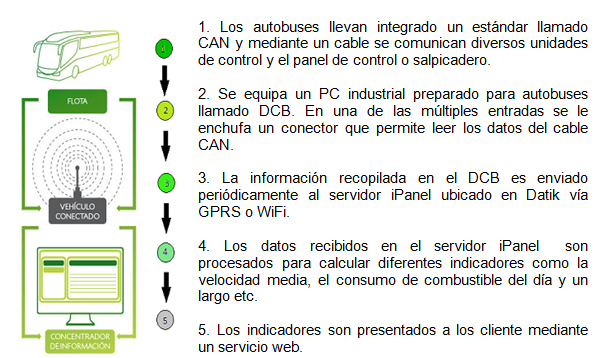
\includegraphics[width=1\textwidth]{Ilustraciones/ipanel_infraesctructure.png}
	\caption{Funcionamiento resumido de iPanel}
	\label{fig:ipanel}
\end{figure}

La incesante integración de nuevos vehículos a iPanel ha generado un crecimiento exponencial en el número de registros almacenados en ciertas tablas de MySQL. Aunque el volumen actual no suponga riesgo alguno para el funcionamiento del servicio, Datik tiene identificados varios escenarios en los que la situación se podría revertir, causando graves problemas en el sistema.\\

El primero de todos, es la corrupción de datos. Este fenómeno sucede debido a un bug, fallo de almacenamiento inesperado, o una caída de MySQL cuando el resultado del checksum de una página es diferente al esperado. Aunque ocurre de forma esporádica, compromete seriamente la información que Datik ofrece a sus clientes mediante la aplicación web.\\ 

Otro de los problemas, intrínseco a depender de una base de datos centralizada, es el operar sobre un único punto de fallo. Debido a que la mayoría de procesos confluyen en ella, el bloqueo o la caída causada por un servicio puede acarrear la de otros, a priori, totalmente independientes. Para solventar el problema Datik ha optado por migrar su infraestructura a una basada en Microservicios \cite{newman2015building}, logrando de esa manera, el aislamiento total de los componentes que conforman su ecosistema.\\ 

El último problema, es el referente al proceso denominado Cálculo de Indicadores, el cual se ejecuta una vez al día para realizar operaciones aritméticas sobre diversas tablas y después agrupa los resultados en base a diferentes criterios dependiendo del cliente. Siendo dichas tablas las que mayor crecimiento experimentan, el aumento del volumen de las mismas incrementa de forma desorbitada el tiempo necesario para finalizar el cálculo, pudiendo, en un futuro, llegar a tardar mas de 24 horas y cancelar los indicadores que ofrecen información del último día.\\

Siendo los indicadores parte vital de la información que se despliega vía iPanel, el presente proyecto ofrece una solución tecnológica para poder escalar horizontalmente la infraestructura solventando así el problema de almacenamiento y ...   

En las proximas lineas se (buscar solucion a los problemas mencionados, sobre todo el ultimo que se encuentra sin solucion visible)

\section{Propuesta}

*la escalabilidad vertical de la máquina no es la solucion viable a largo plazo
*algunos de esos problemas ya empiezan a ser palpables
* problema en el que nos centramos en este proyecto
* requiere de una respuesta tecnologica
* requiere de tecnologia que datik no cuenta

* Palabras de henry ford
* esfuerzo enorme en tunear mysql, no conviene

* Diseccionar el problema: almacenamiento y procesamiento

Para solventar los problemas que Datik prevé, se propone implantar las tecnologías Apache Cassandra y Apache Spark en la empresa y migrar tanto las tablas como los procesos que son parte en el cálculo de los indicadores.\\


Apache Cassandra es una base de datos distribuida no-sql. Gracias a naturaleza distribuida ayuda a resolver, 

Funcionalidades nuevas que trabajan con videos etc




Diseñar un plan de migración que defina aspectos tales como: 

\begin{itemize}
	\item Listado de las tablas MySQL que deben ser migradas a Cassandra priorizando las que más rápido crecen y mayor número de consultas intensivas reciben. Por ejemplo, las tablas que contienen la información para el calculo de los indicadores.
	\item Listado tablas "frontera"
	\item Ver por cada ejercicio su estado de realización: quiénes lo han terminado, quiénes tienen duda y quiénes no han respondido nada.
	\item Editar cualquier detalle de un ejercicio en cualquier momento.
	\item Valorar la realización de un ejercicio a un alumno concreto.
\end{itemize}

el traspaso de las tablas MySQL que mayor velocidad crecen  y mayor número de consultas pesadas reciban a estas nuevas tecnologías. empezando por las que tienen estrecha realción con el calculo de indicadores, ya que, como se ha indicado con anterioridad, es  

Por su parte, Apache Cassandra

Por Apache Spark por otra,

Debido a la falta de datos se ha utilizado un dataset publico para emular las condiciones de futuro con las que se va a encontrar datik

\section{Organización del documento}

En esta memoria se ha documentado  el desarrollo de la herramienta \textbf{\textit{exerClick}}, dentro del Trabajo de Fin de Grado (TFG) del autor. En el documento se describe la propuesta, la planificación y gestión que esta lleva consigo, la implementación llevada a cabo y las conclusiones finales.\\

En este primer capítulo se ha introducido el problema a resolver y se ha explicado la propuesta presentada en este proyecto.\\

En el capítulo 2 se presenta el Documento de Objetivos de Proyecto (DOP). Este recoge el alcance y las fases y tareas del proyecto, el análisis de riesgos y el análisis de factibilidad.\\

Una vez en el capítulo 3 se explica la gestión llevada a cabo durante el proyecto. Se presentan las metodologías utilizadas: Metodologías Ágiles e InterMod (adaptada a las necesidades de este proyecto). A continuación se detallan cada una de las iteraciones llevadas a cabo (como parte de la metodología InterMod): duración, objetivos y tareas realizadas. Al final del capítulo se muestra la documentación asociada a las iteraciones y los objetivos, además del seguimiento de tiempo realizado.\\

A continuación, en el capítulo 4 se detalla el análisis de requisitos. Primero se detallan los requisitos no-funcionales y luego los funcionales (prototipos en papel llevados a cabo durante las primeras iteraciones que dan una visión global del proyecto).\\

En el capítulo 5 se explica el diseño e implementación llevados a cabo. Se comienza mostrando la estructura de documentos del proyecto, luego el diseño realizado en base al análisis de requisitos del capítulo 4 y finalmente una visión general de la implementación de la lógica de negocio.\\

Para finalizar, en el capítulo 6 se presentan las conclusiones, líneas futuras para el proyecto y las lecciones aprendidas.\\

Fuera de la estructura general de la memoria, tenemos la bibliografia y los apéndices. En estos últimos tenemos las actas de reuniones, las actas de pruebas y la vista de relaciones de la base de datos (de la parte utilizada o creada específicamente para el proyecto).\\

%----------------------------------------------------%
%                     OBJETIVOS                      %
%----------------------------------------------------%

%\cleardoublepage
%\input{capitulos/2-objetivos.tex}

%----------------------------------------------------%
%                GESTIÓN DEL PROYECTO                %
%----------------------------------------------------%

%\cleardoublepage
%\input{capitulos/3-gestion.tex}

%----------------------------------------------------%
%              ANALISIS DE REQUISITOS                %
%----------------------------------------------------%

%\cleardoublepage
%\input{capitulos/4-analisis-de-requisitos.tex}

%----------------------------------------------------%
%              DISEÑO E IMPLEMENTACIÓN               %
%----------------------------------------------------%

%\cleardoublepage
%\input{capitulos/5-diseno-e-implementacion.tex}

%----------------------------------------------------%
%                     CONCLUSIONES                   %
%----------------------------------------------------%

%\cleardoublepage
%%----------------------------------------------------%
%                     CONCLUSIONES                   %
%----------------------------------------------------%

\pagestyle{fancy}

\chapter{Conclusiones}
\label{conclusiones}

Tal y como se ha podido apreciar durante el transcurso de la presente tesina, muchas son las ventajas ofrecidas por el uso conjunto de Apache Cassandra y Apache Spark. Entre ellas, cabe resaltar la posibilidad de operar sin punto único de fallo, escalar tanto en almacenamiento como procesamiento prácticamente hasta el infinito y además, mejorar de forma inequívoca, los tiempos de respuesta ofrecidos por MySQL cuando se opera sobre un dataset de volumen considerable.\\

No obstante, existen una seria de inconvenientes a la hora de empezar a gozar de las ventajas descritas en el anterior párrafo.\\

Utilizar este tipo de tecnologías supone un cambio de paradigma enorme en la forma de tratar la información y por ende requiere una inversión de tiempo considerable en la formación del personal y en migrar la arquitectura ya existente.\\

Si de antemano el cambio de paradigma puede repeler a usuarios encallados en bases de datos tradicionales que por diversas circunstancias no encuentran el momento idóneo para dar el salto, la inmadurez de las tecnologías utilizadas en el entorno distribuido no ayuda mucho a disipar las dudas. Al tratarse de software creado recientemente, las actualizaciones son constantes y es difícil mantener una versión estable en entornos de producción.\\

Siguiendo al hilo del mantenimiento, a día de hoy no existe herramienta gratuita alguna que facilite el mantenimiento del clúster, por lo que si no se desea pagar suma elevada de dinero a compañías que ofrecen dicho servicio, es totalmente necesario contar con personal cualificado en mantenimiento de sistemas, algo inviable para empresas pequeñas.\\

En un futuro muy cercano se augura que los inconvenientes recién descritos se irán disipando y que todo tipo de usuario será capaz de sacar provecho a las incuestionables ventajas que ofrecen tanto las tecnologías analizas en presente proyecto, como sus homólogas. No cabe duda alguna que el Big Data es la revolución del presente que impulsa la evolución hacía el futuro.



%----------------------------------------------------%
%                    BIBLIOGRAFIA                    %
%----------------------------------------------------%

%\cleardoublepage
%\nocite{*}
%\printbibliography[heading=bibintoc,title={Bibliografía y Referencias}]

%----------------------------------------------------%
%                    APENDICES                       %
%----------------------------------------------------%

% Reiniciamos el contador de capítulos y hacemos que Capítulo pase a ser Apédice
%\setcounter{chapter}{0}
%\renewcommand{\chaptername}{Apéndice } % dejar el espacio es importante
%\renewcommand{\thechapter}{\Alph{chapter}}

% Cambiamos el titulo para que ponga Apéndice en lugar de Capítulo tal y como acabamos de definir
%\titleformat{\chapter}[display]
%{\normalfont\huge\bfseries}{\chaptername \thechapter}{20pt}{\Huge}[\vspace{2ex}\titlerule]

%\fancyhead[LE,RO]{\itshape \nouppercase \rightmark}
%\fancyhead[LO,RE]{\itshape \nouppercase \chaptername \Alph{chapter}}

%\cleardoublepage
%\input{apendices/a-actas-reuniones.tex}

%\cleardoublepage
%\input{apendices/b-actas-pruebas.tex}

%\cleardoublepage
%\input{apendices/c-base-de-datos.tex}

%\backmatter

\end{document}